\documentclass[t]{beamer}
\mode<presentation>

\usepackage{etex}

\usetheme{Madrid}
% other themes: Warsaw, AnnArbor, Antibes, Bergen, Berkeley, Berlin, Boadilla, boxes, CambridgeUS, Copenhagen, Darmstadt, default, Dresden, Frankfurt, Goettingen,
% Hannover, Ilmenau, JuanLesPins, Luebeck, Madrid, Maloe, Marburg, Montpellier, PaloAlto, Pittsburg, Rochester, Singapore, Szeged, classic

\setbeamertemplate{navigation symbols}{\insertslidenavigationsymbol}

\usecolortheme{dolphin}
%\usecolortheme{seagull}
% color themes: albatross, beaver, beetle, crane, default, dolphin, dov, fly, lily, orchid, rose, seagull, seahorse, sidebartab, structure, whale, wolverine

%\usefonttheme{serif}
% font themes: default, professionalfonts, serif, structurebold, structureitalicserif, structuresmallcapsserif

% pdf is displayed in full screen mode automatically
%\hypersetup{pdfpagemode=FullScreen}

%\AtBeginSection[]
%{
%  \begin{frame}<beamer>
%    \frametitle{Outline}
%    \tableofcontents[currentsection,currentsubsection]
%  \end{frame}
%}

% define your own colors:
\definecolor{Red}{rgb}{1,0,0}
\definecolor{Blue}{rgb}{0,0,1}
\definecolor{Green}{rgb}{0,1,0}
\definecolor{magenta}{rgb}{1,0,.6}
\definecolor{lightblue}{rgb}{0,.8,1}
\definecolor{lightpurple}{rgb}{.6,.4,1}
\definecolor{gold}{rgb}{.6,.5,0}
\definecolor{orange}{rgb}{1,0.4,0}
\definecolor{hotpink}{rgb}{1,0,0.5}
\definecolor{newcolor2}{rgb}{.5,.3,.5}
\definecolor{newcolor}{rgb}{0,.3,1}
\definecolor{newcolor3}{rgb}{1,0,.35}
\definecolor{darkgreen1}{rgb}{0, .35, 0}
\definecolor{darkgreen}{rgb}{0, .4, 0}
\definecolor{medgreen}{rgb}{0, .6, 0}
\definecolor{darkred}{rgb}{.75,0,0}

\xdefinecolor{olive}{cmyk}{0.64,0,0.95,0.4}
\xdefinecolor{purpleish}{cmyk}{0.75,0.75,0,0}

%\usepackage{beamerinnerthemerounded}
% inner themes include circles, default, inmargin, rectangles, rounded

%\usepackage{beamerouterthemesmoothbars}
% outer themes include default, infolines, miniframes, shadow, sidebar, smoothbars, smoothtree, split, tree

\useoutertheme[subsection=false]{smoothbars}

% to have the same footer on all slides
\setbeamertemplate{footline}[text line]{
\raisebox{2pt}{\href{http://www.su.edu}{%
\includegraphics[height=20pt,bb=0 20 234 100,clip]{su.eps}}}\hspace{5pt}
%\raisebox{5pt}{Data Analytics --- May 2018}\hfill
%\raisebox{5pt}{rwojtowi@shepherd.edu}\hfill
%
%  \hspace{-0.2in}\raisebox{10pt}{\color{darkgreen}\href{http://www.adjoint-functors.net/su/web/frf}{www.adjoint-functors.net/su/web/frf}}\hfill\hfill
  \hspace{1in}\raisebox{5pt}{\color{darkgreen}\href{http://www.adjoint-functors.net/su/web/math207}{www.adjoint-functors.net/su/web/math207}\hspace{.2in} {\color{black}2 April 2019}\hfill }
%
%\raisebox{5pt}{\insertframenumber/\pageref{lastpage}}}
\hfill \raisebox{5pt}{\insertframenumber/\inserttotalframenumber}}
%\raisebox{5pt}{\insertframenumber/\insertpresentationendpage}}
%\setbeamertemplate{footline}[text line]{} % or empty footer

% include packages
\usepackage{subfigure}
\usepackage{multicol}
\usepackage{amsmath}
\usepackage{epsfig}
\usepackage{graphicx}
\usepackage[all,knot]{xy}
\xyoption{arc}
\usepackage{url}
\usepackage{multimedia}
\usepackage{hyperref}
\usepackage{setspace}

\title{Hypothesis Testing}
\author{Ralph L. Wojtowicz}
\institute{rlwojtowicz@gmail.com}
\date{\scriptsize 2 April 2019}

\usepackage{pstricks,pst-grad,pst-func,pst-text,pst-node,multido,pst-plot,calc,pst-3dplot,pstricks-add}

\newcommand{\Set}{\ensuremath\mbox{\textbf{Sets}}}

\newcommand{\LOGO}{\href{http://www.su.edu}{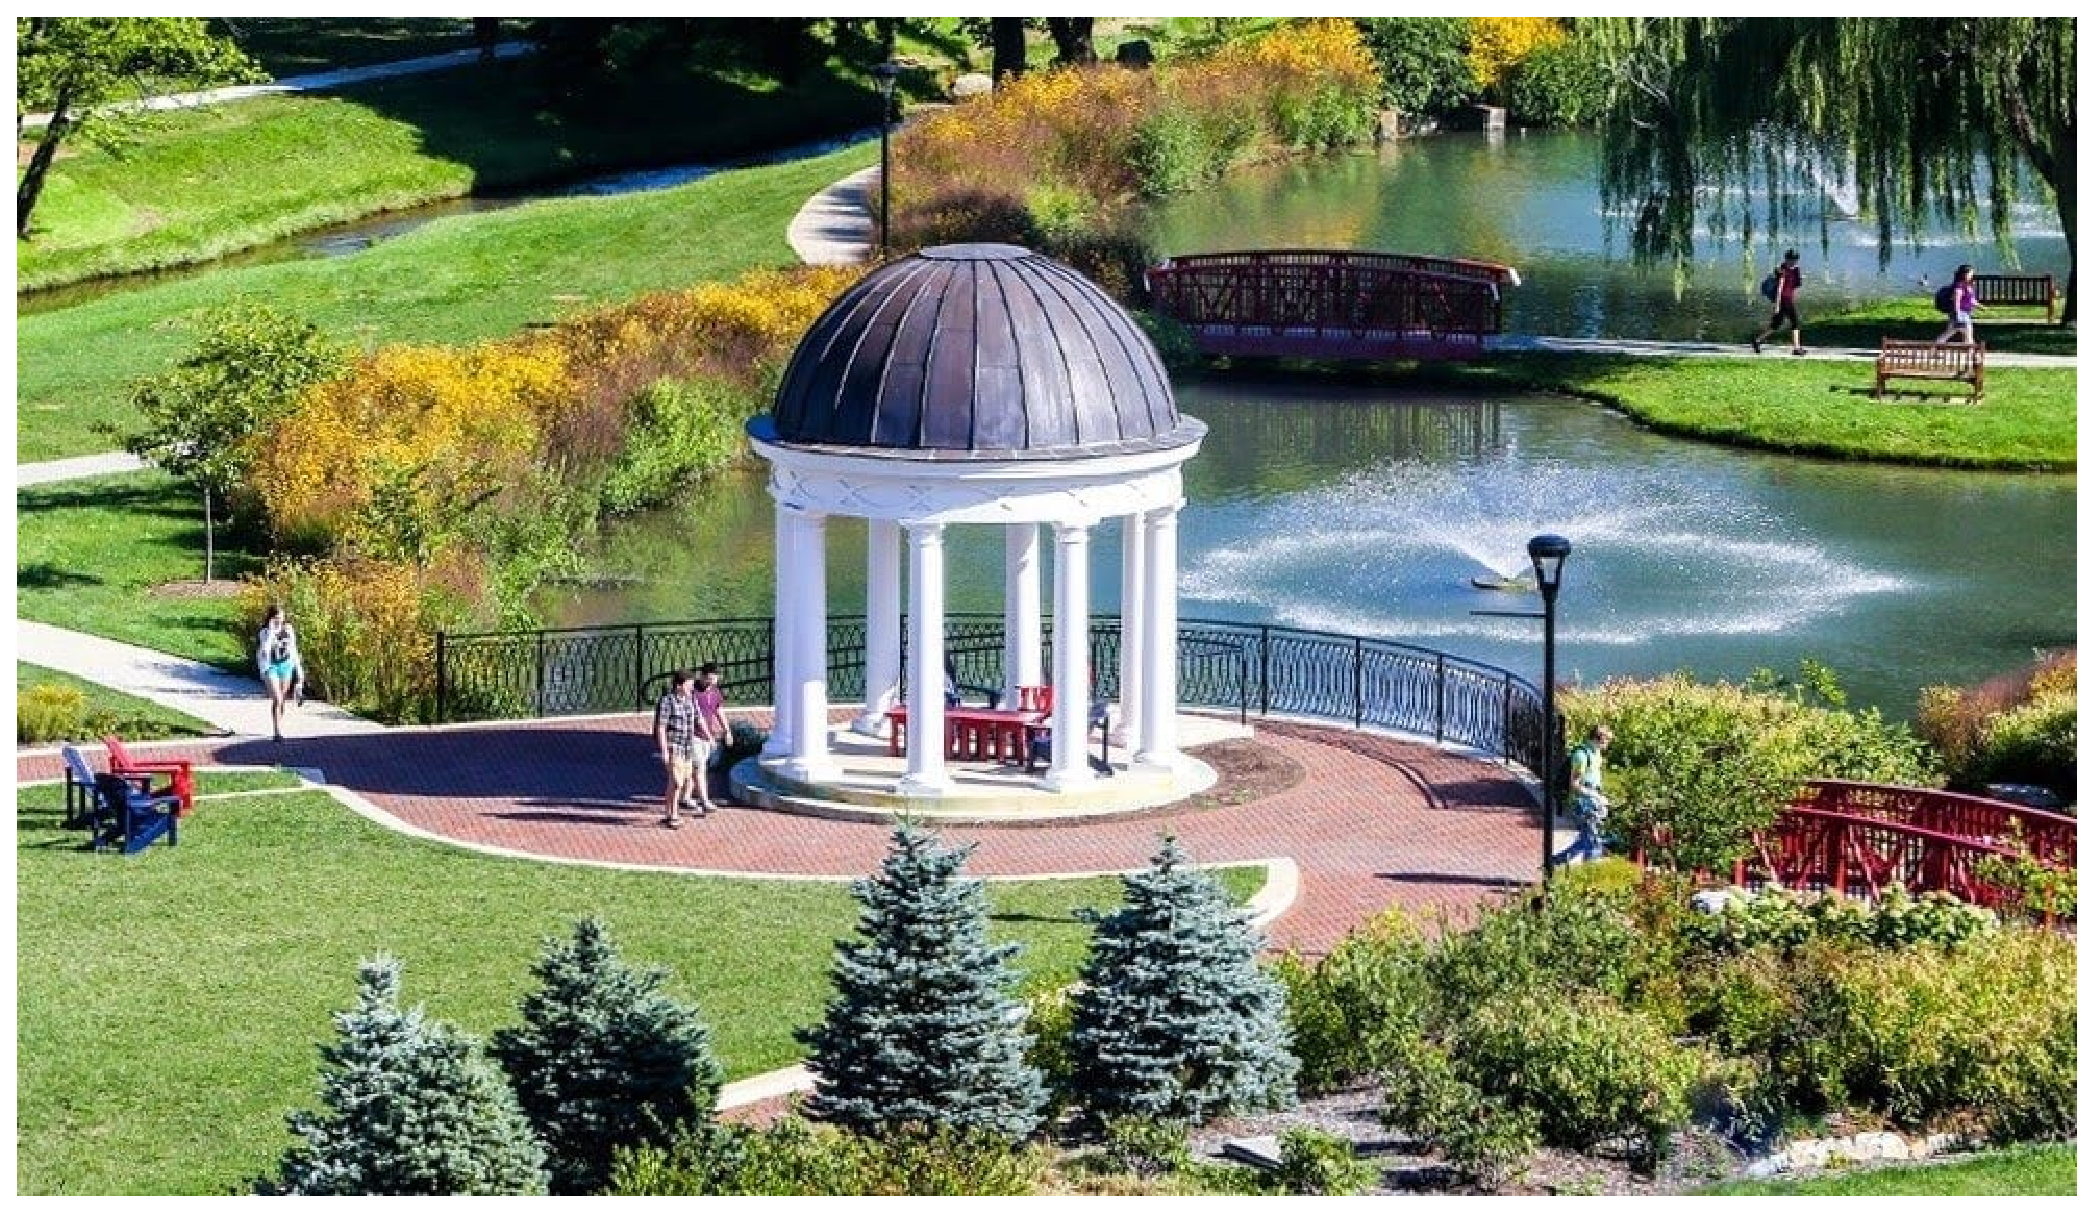
\includegraphics[height=1.3in]{Garden.eps}}}

\newcommand{\US}{%
\large\begin{tabular}{c}
\href{http://www.su.edu}{%
\includegraphics[height=2.1cm,bb=0 20 234 100,clip]{su.eps}} \\[6pt]
\Large Dr.~Ralph L. Wojtowicz \\[6pt]
rwojtowi@su.edu \\[2pt]
%Department of Computers Science, Mathematics and Engineering
\end{tabular}}

\newcommand{\BRACE}{
\begin{pspicture}(-3,-2.1)(3,1.1)
\psset{yunit=3,linewidth=0.02}
\psline(-3.5,0)(3.5,0)  
  \psline(-3,0)(-3,-0.04) \rput[t](-3,-0.07){\scriptsize -3\hphantom{-}}
  \psline(-2,0)(-2,-0.04) \rput[t](-2,-0.07){\scriptsize -2\hphantom{-}}
  \psline(-1,0)(-1,-0.04) \rput[t](-1,-0.07){\scriptsize -1\hphantom{-}}
  \psline(0,0)(0,-0.04)   \rput[t](0,-0.07){\scriptsize 0}
  \psline(1,0)(1,-0.04)   \rput[t](1,-0.07){\scriptsize 1}
  \psline(2,0)(2,-0.04)   \rput[t](2,-0.07){\scriptsize 2}
  \psline(3,0)(3,-0.04)   \rput[t](3,-0.07){\scriptsize 3}
  \rput[l](3.6,0){\scriptsize $x$}
\psline(0,0)(0,0.5)
  \psline(-0.12,0.5)(0,0.5)    \rput[r](-0.21,0.5){\scriptsize $0.5$}
  \psline(-0.12,0.25)(0,0.25)  \rput[r](-0.21,0.25){\scriptsize $0.25$}
\psGauss[linecolor=blue,linewidth=0.02,sigma=1,mue=0]{-3}{3}
\pnode(-1,-0.15){A}\pnode(1,-0.15){B}
\psbrace[braceWidth=0.02,braceWidthInner=5pt,braceWidthOuter=5pt](A)(B){\rput{90}(0.25,-0.05){\scriptsize 68\%}}
%
\pnode(-2,-0.15){C}\pnode(2,-0.15){D}
\psbrace[braceWidth=0.02,braceWidthInner=25pt,braceWidthOuter=5pt](C)(D){\rput{90}(0.25,-0.05){\scriptsize 95\%}}
%
\pnode(-3,-0.15){E}\pnode(3,-0.15){F}
\psbrace[braceWidth=0.02,braceWidthInner=45pt,braceWidthOuter=5pt](E)(F){\rput{90}(0.25,-0.1){\scriptsize 99.7\%}}
\end{pspicture}}

\newcommand{\Z}{\mathbb{Z}}
\newcommand{\N}{\mathbb{N}}

\begin{document}

\AtBeginSection[]
{
%  \begin{frame}<beamer>
%    \frametitle{Outline}
%    \scriptsize
%    \tableofcontents[currentsection,hideothersubsections] %,currentsubsection]
%  \end{frame}
}

%\frame[plain]{
%	\titlepage
%}



\begin{frame}[plain]
\definecolor{myblue}{rgb}{0,0,0.6}
\definecolor{grayA}{rgb}{0.95,0.95,0.95}
\definecolor{grayB}{rgb}{0.98,0.98,0.98}
\begin{center}
%\begin{pspicture}(0,0)(7,4.8)
\begin{pspicture}(-6,-7)(6,2)
\psframe[linewidth=0.02,linecolor=gray](-6.2,-7)(6.2,2.2)
\psframe[linewidth=0.02,linecolor=gray](-6.15,-6.95)(6.15,2.15)


\rput(0,1.4){\color{myblue}\LARGE  Hypothesis Testing}
%\rput(0,0.7){\color{black}\large Faculty Research Forum}
\rput(0,-1.3){\scalebox{1.0}{\LOGO}}
\rput(0,-4.6){\scalebox{.8}{\US}}
\rput(0,-6.6){\scalebox{1.0}{\scriptsize 4 October 2019}}

%\rput(0,-5.95){\scriptsize Dr.\ Ralph L. Wojtowicz}
%\rput(0,-4.25){\scalebox{0.7}{\US}}
%\rput(0,-6.4){\scriptsize 27 October 2014}
\end{pspicture}
\end{center}

\end{frame}

\section{The Normal Curve}
\subsection{Review}
\begin{frame}
\frametitle{The Normal Curve and Standard Units}
{\ }\vspace{-20pt}

{\small

\begin{itemize}
\item The {\color{blue}\textbf{standard normal}}
 (or Gaussian) curve is an ideal histogram to which
  we can compare other data.
\end{itemize}

\begin{center}
\begin{pspicture}(-3,-2.1)(3,0.9)
\psset{yunit=2.5,linewidth=0.02}
\psline(-3.5,0)(3.5,0)  
  \psline(-3,0)(-3,-0.04) \rput[t](-3,-0.07){\scriptsize -3\hphantom{-}}
  \psline(-2,0)(-2,-0.04) \rput[t](-2,-0.07){\scriptsize -2\hphantom{-}}
  \psline(-1,0)(-1,-0.04) \rput[t](-1,-0.07){\scriptsize -1\hphantom{-}}
  \psline(0,0)(0,-0.04)   \rput[t](0,-0.07){\scriptsize 0}
  \psline(1,0)(1,-0.04)   \rput[t](1,-0.07){\scriptsize 1}
  \psline(2,0)(2,-0.04)   \rput[t](2,-0.07){\scriptsize 2}
  \psline(3,0)(3,-0.04)   \rput[t](3,-0.07){\scriptsize 3}
  \rput[l](3.6,0){\scriptsize $z$}
\psline(0,0)(0,0.5)
  \psline(-0.12,0.5)(0,0.5)    \rput[r](-0.21,0.5){\scriptsize $0.5$}
  \psline(-0.12,0.25)(0,0.25)  \rput[r](-0.21,0.25){\scriptsize $0.25$}
\psGauss[linecolor=blue,linewidth=0.02,sigma=1,mue=0]{-3}{3}
\pnode(-1,-0.15){A}\pnode(1,-0.15){B}
\psbrace[braceWidth=0.02,braceWidthInner=5pt,braceWidthOuter=5pt](A)(B){\rput{90}(0.25,-0.05){\scriptsize 68\%}}
%
\pnode(-2,-0.15){C}\pnode(2,-0.15){D}
\psbrace[braceWidth=0.02,braceWidthInner=25pt,braceWidthOuter=5pt](C)(D){\rput{90}(0.25,-0.05){\scriptsize 95\%}}
%
\pnode(-3,-0.15){E}\pnode(3,-0.15){F}
\psbrace[braceWidth=0.02,braceWidthInner=45pt,braceWidthOuter=5pt](E)(F){\rput{90}(0.25,-0.1){\scriptsize 99.7\%}}
\end{pspicture}
\end{center}

\begin{itemize}
\item If $x_1$, $\dots$, $x_n$ is a list of numbers, we convert the values
in the list to {\color{blue}\textbf{standard units}} using the following formula:
\vspace{-2pt}
\end{itemize}
\[z_i = \frac{x_i - \mbox{mean}}{\mbox{SD}}\vspace{-8pt}\]
\begin{itemize}
\item $z_i$ measures how far (in units of SD) $x_i$ is from the mean (average) of the list
\end{itemize}

}
\end{frame}


\subsection{Finding Areas Under the Normal Curve Approximately}
\begin{frame}[t]\frametitle{Finding Areas Under the Normal Curve}

{\small
\begin{itemize}
\item Use one or more of the following to find areas under the normal curve:
  \begin{itemize}
  \item \small Total area under the curve is 1 (that is, 100\%)
  \item \small The area is symmetric about vertical the line $x=0$
  \item \small (area to the left of $x$) $=$ ($1-\mbox{area to the right of $x$}$)
  \item \small The 68\%, 95\%, 99.7\% rules 
  \item \small The \texttt{pnorm} or \texttt{qnorm} functions in \texttt{R} 
   (\href{http://www.r-project.org}{\color{blue}www.r-project.org})
  \item \small Normal tables of values in many statistics textbooks.
 \end{itemize}
\item Example:  
\end{itemize}}

\begin{center}
\begin{pspicture}(-3,-2.5)(3,1.75)
\psframe[linewidth=0.02](-3.8,-1.1)(4.2,1.8)
\psset{yunit=3,linewidth=0.02}
   \pscustom[fillstyle=solid,fillcolor=lightgray,sigma=1,linestyle=none]{
     \psGauss{-3.5}{1.0}
     \psline(1.0, 3.490343)(1.0,0)(-3.5,0) }
   \psGauss[sigma=1,linecolor=blue,linewidth=0.5pt]{-3.5}{3.5}
\psline(1.0,0.24197)(1.0,0)   %\rput[t](1.25,-0.25){\scriptsize 1.25}
\rput[l](1.5,0.3){\scriptsize$\mbox{\texttt{area}} = \frac{68\%}{2}=34\%$}
\psline{->}(1.45,0.29)(0.5,0.15)
%
\rput[r](-1.5,0.3){\scriptsize$\mbox{\texttt{area}} = 50\%$}
\psline{->}(-1.45,0.29)(-0.5,0.15)
%
\psline(-3.5,0)(3.5,0)  
  \psline(-3,0)(-3,-0.04) \rput[t](-3,-0.07){\scriptsize -3\hphantom{-}}
  \psline(-2,0)(-2,-0.04) \rput[t](-2,-0.07){\scriptsize -2\hphantom{-}}
  \psline(-1,0)(-1,-0.04) \rput[t](-1,-0.07){\scriptsize -1\hphantom{-}}
  \psline(0,0)(0,-0.04)   \rput[t](0,-0.07){\scriptsize 0}
  \psline(1,0)(1,-0.04)   \rput[t](1,-0.07){\scriptsize 1}
  \psline(2,0)(2,-0.04)   \rput[t](2,-0.07){\scriptsize 2}
  \psline(3,0)(3,-0.04)   \rput[t](3,-0.07){\scriptsize 3}
  \rput[l](3.6,0){\scriptsize $z$}
\psline(0,0)(0,0.5)
  \psline(-0.12,0.5)(0,0.5)    \rput[r](-0.21,0.5){\scriptsize $0.5$}
  \psline(-0.12,0.25)(0,0.25)  \rput[r](-0.21,0.25){\scriptsize $0.25$}
\rput(0,-0.24){\footnotesize $\mbox{Total area} = 50\% + 34\% = 84\%$}
\end{pspicture}
\end{center}

\end{frame}

\subsection{Finding Areas Under the Normal Curve with \texttt{R}}
\begin{frame}[t]\frametitle{Finding Areas Under the Normal Curve with \texttt{R}}

\begin{center}
\scalebox{0.7}{\begin{tabular}{ccc}
\begin{pspicture}(-3,-2.5)(4,1.75)
\psframe[linewidth=0.02](-3.8,-1.1)(4.2,1.8)
\psset{yunit=3,linewidth=0.02,arrowsize=3pt 2}
%
   \pscustom[fillstyle=solid,fillcolor=lightgray,sigma=1,linestyle=none]{
     \psGauss{-3.5}{1.25}
     \psline(1.25, 3.490343)(1.25,0)(-3.5,0) }
   \psGauss[sigma=1,linecolor=blue,linewidth=0.5pt]{-3.5}{3.5}
\psline(1.25,0.1826)(1.25,-0.22)   \rput[t](1.25,-0.25){\scriptsize 1.25}
\rput[l](1.5,0.3){\scriptsize\texttt{pnorm}$(1.25)\approx 0.894$}
\psline{->}(1.45,0.29)(0.5,0.2)
%
\psline(-3.5,0)(3.5,0)  
  \psline(-3,0)(-3,-0.04) \rput[t](-3,-0.07){\scriptsize -3\hphantom{-}}
  \psline(-2,0)(-2,-0.04) \rput[t](-2,-0.07){\scriptsize -2\hphantom{-}}
  \psline(-1,0)(-1,-0.04) \rput[t](-1,-0.07){\scriptsize -1\hphantom{-}}
  \psline(0,0)(0,-0.04)   \rput[t](0,-0.07){\scriptsize 0}
  \psline(1,0)(1,-0.04)   \rput[t](1,-0.07){\scriptsize 1}
  \psline(2,0)(2,-0.04)   \rput[t](2,-0.07){\scriptsize 2}
  \psline(3,0)(3,-0.04)   \rput[t](3,-0.07){\scriptsize 3}
  \rput[l](3.6,0){\scriptsize $x$}
\psline(0,0)(0,0.5)
  \psline(-0.12,0.5)(0,0.5)    \rput[r](-0.21,0.5){\scriptsize $0.5$}
  \psline(-0.12,0.25)(0,0.25)  \rput[r](-0.21,0.25){\scriptsize $0.25$}
\end{pspicture}
&
&
\begin{pspicture}(-4,-2.5)(3,1.75)
\psframe[linewidth=0.02](-3.8,-1.1)(4.2,1.8)
\psset{yunit=3,linewidth=0.02,arrowsize=3pt 2}
%
   \pscustom[fillstyle=solid,fillcolor=lightgray,sigma=1,linestyle=none]{
     \psGauss{-0.5}{1.25}
     \psline(1.25, 3.490343)(1.25,0)(-0.5,0)(-0.5,0.352065)}
   \psGauss[sigma=1,linecolor=blue,linewidth=0.5pt]{-3.5}{3.5}
\psline(1.25,0.1826)(1.25,-0.22)   \rput[t](1.25,-0.25){\scriptsize 1.25}
\psline(-0.5,0.352065)(-0.5,-0.22)   \rput[t](-0.5,-0.25){\scriptsize $-0.5$}
\rput[l](0.8,0.45){\scriptsize$\mbox{\texttt{pnorm}}(1.25)-\mbox{\texttt{pnorm}}(-0.5)$}
\rput[l](2.5,0.33){\scriptsize$\approx 0.586$}
\psline{->}(2.1,0.32)(0.5,0.1)
%
\psline(-3.5,0)(3.5,0)  
  \psline(-3,0)(-3,-0.04) \rput[t](-3,-0.07){\scriptsize -3\hphantom{-}}
  \psline(-2,0)(-2,-0.04) \rput[t](-2,-0.07){\scriptsize -2\hphantom{-}}
  \psline(-1,0)(-1,-0.04) \rput[t](-1,-0.07){\scriptsize -1\hphantom{-}}
  \psline(0,0)(0,-0.04)   \rput[t](0,-0.07){\scriptsize 0}
  \psline(1,0)(1,-0.04)   \rput[t](1,-0.07){\scriptsize 1}
  \psline(2,0)(2,-0.04)   \rput[t](2,-0.07){\scriptsize 2}
  \psline(3,0)(3,-0.04)   \rput[t](3,-0.07){\scriptsize 3}
  \rput[l](3.6,0){\scriptsize $x$}
\psline(0,0)(0,0.5)
  \psline(-0.12,0.5)(0,0.5)    \rput[r](-0.21,0.5){\scriptsize $0.5$}
  \psline(-0.12,0.25)(0,0.25)  \rput[r](-0.21,0.25){\scriptsize $0.25$}
\end{pspicture}\\[-30pt]
%%
%%
\begin{pspicture}(-3,-2.5)(4,1.75)
\psframe[linewidth=0.02](-3.8,-1.1)(4.2,1.8)
\psset{yunit=3,linewidth=0.02,arrowsize=3pt 2}
%
   \pscustom[fillstyle=solid,fillcolor=lightgray,sigma=1,linestyle=none]{
     \psGauss{3.5}{1.25}
     \psline(1.25, 3.490343)(1.25,0)(3.5,0) }
   \psGauss[sigma=1,linecolor=blue,linewidth=0.5pt]{-3.5}{3.5}
\psline(1.25,0.1826)(1.25,-0.22)   \rput[t](1.25,-0.25){\scriptsize 1.25}
\rput[l](0.8,0.38){\scriptsize$1-\mbox{\texttt{pnorm}}(1.25)\approx 0.106$}
\psline{->}(1.45,0.29)(1.5,0.04)
%
\psline(-3.5,0)(3.5,0)  
  \psline(-3,0)(-3,-0.04) \rput[t](-3,-0.07){\scriptsize -3\hphantom{-}}
  \psline(-2,0)(-2,-0.04) \rput[t](-2,-0.07){\scriptsize -2\hphantom{-}}
  \psline(-1,0)(-1,-0.04) \rput[t](-1,-0.07){\scriptsize -1\hphantom{-}}
  \psline(0,0)(0,-0.04)   \rput[t](0,-0.07){\scriptsize 0}
  \psline(1,0)(1,-0.04)   \rput[t](1,-0.07){\scriptsize 1}
  \psline(2,0)(2,-0.04)   \rput[t](2,-0.07){\scriptsize 2}
  \psline(3,0)(3,-0.04)   \rput[t](3,-0.07){\scriptsize 3}
  \rput[l](3.6,0){\scriptsize $x$}
\psline(0,0)(0,0.5)
  \psline(-0.12,0.5)(0,0.5)    \rput[r](-0.21,0.5){\scriptsize $0.5$}
  \psline(-0.12,0.25)(0,0.25)  \rput[r](-0.21,0.25){\scriptsize $0.25$}
\end{pspicture}
&
&
\begin{pspicture}(-4,-2.5)(3,1.75)
\psframe[linewidth=0.02](-3.8,-1.1)(4.2,1.8)
\psset{yunit=3,linewidth=0.02,,arrowsize=3pt 2}
%
   \pscustom[fillstyle=solid,fillcolor=lightgray,sigma=1,linestyle=none]{
     \psGauss{-3.5}{0.6744898}
     \psline(0.6744898, 0.3177766)(0.6744898,0)(-3.5,0) }
   \psGauss[sigma=1,linecolor=blue,linewidth=0.5pt]{-3.5}{3.5}
\psline(0.6744898,0.3177766)(0.6744898,-0.22)   
   \rput[tl](0.61,-0.23){\scriptsize\texttt{qnorm}$(0.75)\approx 0.67$}
\rput[l](1.5,0.3){\scriptsize$\mbox{area}=0.75$}
\psline{->}(1.45,0.29)(0.25,0.15)
%
\psline(-3.5,0)(3.5,0)  
  \psline(-3,0)(-3,-0.04) \rput[t](-3,-0.07){\scriptsize -3\hphantom{-}}
  \psline(-2,0)(-2,-0.04) \rput[t](-2,-0.07){\scriptsize -2\hphantom{-}}
  \psline(-1,0)(-1,-0.04) \rput[t](-1,-0.07){\scriptsize -1\hphantom{-}}
  \psline(0,0)(0,-0.04)   \rput[t](0,-0.07){\scriptsize 0}
  \psline(1,0)(1,-0.04)   \rput[t](1,-0.07){\scriptsize 1}
  \psline(2,0)(2,-0.04)   \rput[t](2,-0.07){\scriptsize 2}
  \psline(3,0)(3,-0.04)   \rput[t](3,-0.07){\scriptsize 3}
  \rput[l](3.6,0){\scriptsize $x$}
\psline(0,0)(0,0.5)
  \psline(-0.12,0.5)(0,0.5)    \rput[r](-0.21,0.5){\scriptsize $0.5$}
  \psline(-0.12,0.25)(0,0.25)  \rput[r](-0.21,0.25){\scriptsize $0.25$}
\end{pspicture}
\end{tabular}}
\end{center}


\end{frame}


\section{The $z$-Test}
\subsection{The $z$-Test}
\begin{frame}
\frametitle{Drs.\ Nullsheimer and Altshuler Debate the Contents of a Box of Numbered Tickets }
{\ }\vspace{-25pt}

{\footnotesize
\begin{itemize}
\item Drs.\ Nullsheimer and Altshuler are arguing about a large box of numbered tickets.  
\item Dr.\ Null says that the average is 50.  
\item Dr.\ Alt says the average is different from 50.
\item They get tired of arguing and decide to look at some data.
\item They draw a random sample of 500 tickets (with replacement).  
\item The average of the draws turns out to be 48 and the SD is 15.3.
\end{itemize}
\smallskip

\begin{tabular}{ll}
{\color{blue}Dr.\ Alt} & {\color{blue}The average is really below 50.}\\
Dr.\ Null &Oh, come on, the difference is only 2, and the SD is 15.3.  The difference \\  & 
   is tiny relative to the SD.  It's just chance.\\
{\color{blue}Dr.\ Alt} & {\color{blue}Hmmm. Dr.\ Nullsheimer, I think we need to look at the SE, not the SD.}\\
Dr.\ Null & Why is that?\\
{\color{blue}Dr.\ Alt} & {\color{blue}Because the SE tells us how far the average of the sample is likely to be } \\ &
   {\color{blue}from its expected value --- the average of the box.}\\
Dr.\ Null & So, what's the SE?\\
{\color{blue}Dr.\ Alt} & {\color{blue}Can we agree to estimate the SD of the box as 15.3, the SD of the data?}\\
Dr.\ Null & I'll go along with you there.\\
\end{tabular}}
\end{frame}

\begin{frame}
\frametitle{Debate (continued) }
{\ }

{\footnotesize
\begin{tabular}{ll}
{\color{blue}Dr.\ Alt} & {\color{blue}OK, then the SE for the average of the draws is about $15.3/\sqrt{500} \approx 0.7$.}\\[2pt]
Dr.\ Null & So?\\[2pt]
{\color{blue}Dr.\ Alt} & {\color{blue}The average of the draws is 48.  You say it ought to be 50.  If your theory}  \\ 
    & {\color{blue}is right, the average is about 3 SEs below its expected value.}\\[2pt]
Dr.\ Null & Where did you get the 3?\\[5pt]
{\color{blue}Dr.\ Alt} & {\color{blue}Well, }
{\color{blue} $\displaystyle z = 
     \frac{\mbox{\footnotesize observed value} -
     \mbox{\footnotesize expected value}}{\mbox{\footnotesize standard error}}
      = \frac{48-50}{0.7}\approx -3$}\vspace{5pt}
\\[5pt]
Dr.\ Null & You're going to tell me that 3 SEs is too many SEs to explain by chance?\\[2pt]
{\color{blue}Dr.\ Alt} & {\color{blue}That's my point.  You can't explain the difference by chance.}  
   \\ & {\color{blue}The difference is real.  In other words, the average of the tickets in the box}\\
   & {\color{blue}isn't 50, it's some other number.}\\[2pt]
Dr.\ Null & I thought the SE was about the difference between the sample average \\ & 
    and its expected value.\\[2pt]
{\color{blue}Dr.\ Alt}  & {\color{blue}Yes, yes.  But the expected value of the sample average \textit{is} the} \\ & 
     {\color{blue}average of the tickets in the box.}
\end{tabular}}
\end{frame}


\subsection{Central Limit Theorem}
\begin{frame}
\frametitle{The Central Limit Theorem}

When drawing at random with replacement from a box, the probability histogram for the sum
(and the average)
will follow the normal curve, even if the contents of the box do not.  The histogram
must be put into standard units, and the number of draws must be reasonably large.\vspace{-8pt}

\begin{center}
{\setlength{\tabcolsep}{2pt}\begin{tabular}{ccccccc}
$\displaystyle\mbox{EV}_{\mbox{\scriptsize sum}}$ & $=$  & $n\cdot \mbox{AV}_{\mbox{\scriptsize box}}$ & 
   \hspace{.5in}
$\displaystyle\mbox{EV}_{\mbox{\scriptsize av}}$ &  $=$ & $\hphantom{n\cdot }\mbox{AV}_{\mbox{\scriptsize box}}$ \\[5pt]
%
$\displaystyle\mbox{SE}_{\mbox{\scriptsize sum}}$ & $=$ & $\sqrt{n}\cdot \mbox{SD}_{\mbox{\scriptsize box}}$ & 
   \hspace{.5in}
$\displaystyle\mbox{SE}_{\mbox{\scriptsize av}}$  & $=$ & 
  $\frac{\mbox{SD}_{\mbox{\tiny box}}}{\sqrt{n}}$ \\
\end{tabular}}

\begin{tabular}{ccc}
\begin{pspicture}(-3,0)(2,2.5)
\psframe(-3,-1.0)(2.4,2.3)
\psGauss[linecolor=red,mue=-1,sigma=0.4]{-3}{2}
\psGauss[linecolor=blue,mue=-0.5, sigma=0.5]{-2.5}{2}
\psGauss[linecolor=black,mue=0, sigma=0.6]{-2}{2}
\psline{->}(-1,-0.3)(1,-0.3)
\rput(0,-0.6){increasing $n$}
\end{pspicture}
& \hspace{.2in}
\begin{pspicture}(-2,0)(2,2.5)
\psframe(-2.3,-1.0)(2.3,2.3)
\psGauss[linecolor=red,mue=0,sigma=0.4]{-2}{2}
\psGauss[linecolor=blue,mue=0, sigma=0.3]{-2}{2}
\psGauss[linecolor=black,mue=0, sigma=0.2]{-2}{2}
\psline{->}(1.2,0.3)(1.2,1.9)
\rput{90}(1.5,1.12){increasing $n$}
\end{pspicture}

\end{tabular}
\end{center}
  
\end{frame}


\subsection{Variations  on the Dialog Example}
\begin{frame}
\frametitle{Variations on the Dialog Example}

{\small\begin{enumerate}
\item In the dialog, suppose the 500 tickets in the sample average 48 but\\ the SD is 33.6.  
Who wins?\vspace{-5pt}
\[\mbox{SE}_{\mbox{\scriptsize av}} = \frac{33.6}{\sqrt{500}} \approx 1.5
\hspace{.5in} \mbox{and}\hspace{.5in}
  z = \frac{48-50}{1.5}= -1.3\vspace{-5pt}\]
\item  Suppose 100 tickets are drawn, not 500, the sample average is $48$ and\\ the SD is $33.6$.
Who wins?\vspace{-5pt}
\[\mbox{SE}_{\mbox{\scriptsize av}} = \frac{33.6}{\sqrt{100}} \approx 3.36
\hspace{.5in} \mbox{and}\hspace{.5in}
  z = \frac{48-50}{3.36}= -0.59\]
\item Suppose 10,000 tickets are drawn, the sample average is $50.3$ and \\ the SD is 15.  
Who wins?\vspace{-5pt}
\[\mbox{SE}_{\mbox{\scriptsize av}} = \frac{15.0}{\sqrt{10,000}} = 0.15
\hspace{.5in} \mbox{and}\hspace{.5in}
  z = \frac{50.3-50}{0.15}= 2\]
\end{enumerate}
}
\end{frame}

\subsection{Hypothesis Testing}
\begin{frame}
\frametitle{Hypothesis Testing}
{%\small

\begin{itemize}
\item \textbf{\color{blue}Null Hypothesis}:  The difference between the expected and observed
values is due to chance.
\item \textbf{\color{blue}Alternative Hypothesis}:  No it's not!
\item \textbf{\color{blue}$p$-Value}:  If we assume that the null hypothesis is true, what is
the chance of getting data as extreme or more extreme than the observed values?
\item \textbf{\color{blue}Examples}:\vspace{-1pt}
\begin{center}
\begin{tabular}{ccl}
   $P(z < -3.00) \approx \hphantom{0}0.1\%$ & highly significant! & Accept Alternative\\[5pt]
   $P(z < -1.30) \approx \hphantom{0}9.7\%$ &  & Accept Null\\[5pt]
   $P(z < -0.59) \approx 27.8\%$            &  & Accept Null\\[5pt]
   $P(z > -2.00) \approx \hphantom{0}2.3\%$       & significant & Accept Alternative 
\end{tabular}
\end{center}
\item \textbf{Small $p$-values support the alternative hypothesis.}
\end{itemize}

}

\end{frame}

\subsection{Coin-Tossing Example}
\begin{frame}
\frametitle{Coin-Tossing Example}

{\small 
A coin is tossed 10,000 times, and it lands heads 5,167 times.  Is the chance of heads equal to 50\%?

\begin{itemize}
\item \textbf{\color{blue}Null Hypothesis}:  The coin is fair.  The observed percentage 51.67\% differs
from the expected value 50.0\% due to chance.
\item \textbf{\color{blue}Alternative Hypothesis}: No, it's not fair!
\item \textbf{\color{blue}Box model}: \psframebox{\;0\hspace{20pt} 1\;}
\item $\mbox{AV}_{\mbox{\scriptsize box}} = 0.5$ \hspace{.5in} 
   $\mbox{SD}_{\mbox{\scriptsize box}} = 0.5$ 
\item $\mbox{EV}_{\mbox{\scriptsize av}} = 50\%$ \hspace{.5in}
   $\mbox{SE}_{\mbox{\scriptsize av}} = \frac{0.5}{\sqrt{10,000}}= 0.5\%$ 
\item Test statistic $\displaystyle z=\frac{51.67 - 50.0}{0.5} \approx 3.3$
\item \textbf{\color{blue}$p$-value} $=$ area to the right of 3.3 under the normal curve $\approx 0.05\%$
\item \textbf{\color{blue}Conclusion}:  the coin is (very likely) not fair!
\end{itemize}
}

\end{frame}


\section{The $t$-Test}
\subsection{The $t$-Test}
\begin{frame}
\frametitle{The $t$-Distribution and $t$-Test}
{\ }\vspace{-20pt}
{\small 

\begin{itemize}
\item The {\color{blue}Central Limit Theorem} asserts that the sum (or average) of a random sample
   follows the normal curve {\color{blue}if the sample size is reasonably large}.
\item If the sample size is small, then the appropriate probability distribution 
(ideal histogram) is a {\color{blue}$t$-distribution}.
\item A $t$-distribution is similar to the normal curve but it is flatter in the middle and
   allows a bit more probability for extreme values.
\item A $t$-distribution has a parameter called {\color{blue}degrees of freedom (DOF)}  
$= n-1$ which influences its shape.
\item As DOF increases, the $t$-distribution looks more like the  normal curve.
\end{itemize}}

\begin{center}
\begin{pspicture}(-3,-2.0)(3,2.0)
\psframe[linewidth=0.02](-3.8,-0.6)(4.2,2.0)
\psset{yunit=3.5,linewidth=0.02}
\psGauss[sigma=1,linecolor=black,linewidth=0.5pt]{-3.5}{3.5}
\psTDist[nue=2,linecolor=green,linewidth=0.5pt]{-3.5}{3.5}
\psTDist[nue=6,linecolor=blue,linewidth=0.5pt]{-3.5}{3.5}
%
\psline(-3.5,0)(3.5,0)  
  \psline(-3,0)(-3,-0.04) \rput[t](-3,-0.07){\scriptsize -3\hphantom{-}}
  \psline(-2,0)(-2,-0.04) \rput[t](-2,-0.07){\scriptsize -2\hphantom{-}}
  \psline(-1,0)(-1,-0.04) \rput[t](-1,-0.07){\scriptsize -1\hphantom{-}}
  \psline(0,0)(0,-0.04)   \rput[t](0,-0.07){\scriptsize 0}
  \psline(1,0)(1,-0.04)   \rput[t](1,-0.07){\scriptsize 1}
  \psline(2,0)(2,-0.04)   \rput[t](2,-0.07){\scriptsize 2}
  \psline(3,0)(3,-0.04)   \rput[t](3,-0.07){\scriptsize 3}
  \rput[l](3.6,0){\scriptsize $z$}
\psline(0,0)(0,0.5)
  \psline(-0.12,0.5)(0,0.5)    \rput[r](-0.21,0.5){\scriptsize $0.5$}
  \psline(-0.12,0.25)(0,0.25)  \rput[r](-0.21,0.25){\scriptsize $0.25$}
\end{pspicture}
\end{center}
\end{frame}


\subsection{Spectrophotometer I}
\begin{frame}
\frametitle{Spectrophotometer Example I}

{\small

A spectrophotometer is a device that can be used to detect concentrations of 
pollutants (such as CO) in air samples.  
A  spectrophotometer is being calibrated with a manufactured sample.  
The technician makes five readings and gets\vspace{-4pt}
\[78 \hspace{.2in} 83\hspace{.2in} 68\hspace{.2in} 72\hspace{.2in} 88\vspace{-4pt}\]
measured in ppm.  If the device is working correctly, the expected value is 70.
\begin{itemize}
\item \textbf{\color{blue}Box model}: $\mbox{measurement} = \mbox{true value}\; +\; \mbox{bias}\; + \;
     \mbox{\color{blue}chance error}$
\item  Sample average $=$ 77.8
\item  Sample SD $=$ 8.1
\item  $\mbox{SE}_{\mbox{\scriptsize av}} = \frac{8.1}{\sqrt{4}} = 4.05$
\item test statistic $\displaystyle z =\frac{77.8 - 70}{4.05} \approx 1.92$
\item \textbf{\color{blue}$p$-Value}: area to the right of 1.92 under the $t$-distribution with $5-1 = 4$
     degrees of freedom $=$ 6.3\%
\item \textbf{\color{blue}Conclusion}: (Hesitantly) accept the null hypothesis.
\end{itemize}}

\end{frame}

\subsection{Spectrophotometer II}
\begin{frame}
\frametitle{Spectrophotometer Example II}

{\small

Suppose the technician makes only three readings which are\vspace{-5pt}
\[71 \hspace{.4in} 68\hspace{.4in} 79\vspace{-8pt}\]
measured in ppm.  Is the device working correctly?
\begin{itemize}
\item  Sample average $=$ 72.7
\item  Sample SD $=$ 5.7
\item  $\mbox{SE}_{\mbox{\scriptsize av}} = \frac{5.7}{\sqrt{3}} = 3.3$
\item test statistic $\displaystyle z =\frac{72.7 - 70}{3.3} \approx 0.82$
\item \textbf{\color{blue}$p$-Value}: area to the right of 0.82 under the $t$-distribution with $3-1 = 2$
     degrees of freedom $=$ 25\%
\item \textbf{\color{blue}Conclusion}: Accept the null hypothesis.
\end{itemize}}

\end{frame}

\section{The Two-Sample $z$-Test}
\subsection{The Two-Sample $z$-Test I}
\begin{frame}
\frametitle{Two-Sample $z$-Test (I)}
{\small

400 draws are made at random with replacement from box $A$. The sample average and SD are 110 and 60.
Independently, 100 draws are made at random with replacement from box $B$.  
The sample average and SD are 90 and 40.  Are the averages of the tickets in the two boxes equal?

\begin{itemize}
\item \textbf{\color{blue}Null Hypothesis}:  The boxes have the same average.  
   The observed difference is simply due to chance.
\item \textbf{\color{blue}Alternative Hypothesis}: No, it's not!
\item $\mbox{SE}_{A} = \frac{60}{\sqrt{400}}=3$ \hspace{.5in}
   $\mbox{SE}_{B} = \frac{40}{\sqrt{100}}= 4$
\item $\mbox{SE}_{\mbox{\scriptsize diff}} = \sqrt{3^2 + 4^2} = 5$.
\item $\displaystyle z=\frac{\mbox{\footnotesize observed difference} -
     \mbox{\footnotesize expected difference}}{\mbox{\footnotesize standard error}} = 
\frac{(110 - 90)\; -\; 0}{5} = 4$
\item \textbf{\color{blue}$p$-value} $=$ area to the right of 4 under the normal curve $\approx 0.0032\%$
\item \textbf{\color{blue}Conclusion}:  The averages are very likely \textbf{not} the same.
\end{itemize}
}
\end{frame}

\subsection{The Two-Sample $z$-Test II}
\begin{frame}
\frametitle{Two-Sample $z$-Test (II)}

{Repeat the last example but assume that the sample sizes were both 50.

\begin{itemize}
\item \textbf{\color{blue}Null Hypothesis}:  The boxes have the same average.  
   The observed difference is simply due to chance.
\item \textbf{\color{blue}Alternative Hypothesis}: No, it's not!\vspace{3pt}
\item $\mbox{SE}_{A} = \frac{60}{\sqrt{50}}=8.5$ \hspace{.5in}
   $\mbox{SE}_{B} = \frac{40}{\sqrt{50}}\approx 5.7$\vspace{3pt}
\item $\mbox{SE}_{\mbox{\scriptsize diff}} = \sqrt{8.5^2 + 5.7^2}\approx 10.2$.\vspace{3pt}
\item $\displaystyle z=
    \frac{(110 - 90)\; -\; 0}{10.2} = 1.96$\vspace{3pt}
\item \textbf{\color{blue}$p$-value} $=$ area to the right of 1.96 under the normal curve $\approx 2.5\%$
\vspace{3pt}
\item \textbf{\color{blue}Conclusion}:  The averages are  likely \textbf{not} the same.
\end{itemize}
}
\end{frame}
\end{document}

{\small

\begin{center}
\begin{pspicture}(-3,-2.5)(3,1.75)
\psframe[linewidth=0.02](-3.8,-1.1)(4.2,1.8)
\psset{yunit=3,linewidth=0.02}
%
   \pscustom[fillstyle=solid,fillcolor=lightgray,sigma=1,linestyle=none]{
     \psGauss{-3.5}{1.25}
     \psline(1.25, 3.490343)(1.25,0)(-3.5,0) }
   \psGauss[sigma=1,linecolor=blue,linewidth=0.5pt]{-3.5}{3.5}
\psline(1.25,0.1826)(1.25,-0.22)   \rput[t](1.25,-0.25){\scriptsize 1.25}
\rput[l](1.5,0.3){\scriptsize\texttt{pnorm}$(1.25)\approx 0.894$}
\psline{->}(1.45,0.29)(0.5,0.2)
%
\psline(-3.5,0)(3.5,0)  
  \psline(-3,0)(-3,-0.04) \rput[t](-3,-0.07){\scriptsize -3\hphantom{-}}
  \psline(-2,0)(-2,-0.04) \rput[t](-2,-0.07){\scriptsize -2\hphantom{-}}
  \psline(-1,0)(-1,-0.04) \rput[t](-1,-0.07){\scriptsize -1\hphantom{-}}
  \psline(0,0)(0,-0.04)   \rput[t](0,-0.07){\scriptsize 0}
  \psline(1,0)(1,-0.04)   \rput[t](1,-0.07){\scriptsize 1}
  \psline(2,0)(2,-0.04)   \rput[t](2,-0.07){\scriptsize 2}
  \psline(3,0)(3,-0.04)   \rput[t](3,-0.07){\scriptsize 3}
  \rput[l](3.6,0){\scriptsize $z$}
\psline(0,0)(0,0.5)
  \psline(-0.12,0.5)(0,0.5)    \rput[r](-0.21,0.5){\scriptsize $0.5$}
  \psline(-0.12,0.25)(0,0.25)  \rput[r](-0.21,0.25){\scriptsize $0.25$}
\end{pspicture}
%%%
\begin{pspicture}(-3,-2.1)(3,1.1)
\psframe[linewidth=0.02](-3.8,-1.1)(4.2,1.8)
\psset{yunit=3,linewidth=0.02}
%
   \pscustom[fillstyle=solid,fillcolor=lightgray,sigma=1,linestyle=none]{
     \psGauss{-3.5}{0.6744898}
     \psline(0.6744898, 0.3177766)(0.6744898,0)(-3.5,0) }
   \psGauss[sigma=1,linecolor=blue,linewidth=0.5pt]{-3.5}{3.5}
\psline(0.6744898,0.3177766)(0.6744898,-0.22)   
   \rput[tl](0.61,-0.23){\scriptsize\texttt{qnorm}$(0.75)\approx 0.67$}
\rput[l](1.5,0.3){\scriptsize$\mbox{area}=0.75$}
\psline{->}(1.45,0.29)(0.25,0.15)
%
\psline(-3.5,0)(3.5,0)  
  \psline(-3,0)(-3,-0.04) \rput[t](-3,-0.07){\scriptsize -3\hphantom{-}}
  \psline(-2,0)(-2,-0.04) \rput[t](-2,-0.07){\scriptsize -2\hphantom{-}}
  \psline(-1,0)(-1,-0.04) \rput[t](-1,-0.07){\scriptsize -1\hphantom{-}}
  \psline(0,0)(0,-0.04)   \rput[t](0,-0.07){\scriptsize 0}
  \psline(1,0)(1,-0.04)   \rput[t](1,-0.07){\scriptsize 1}
  \psline(2,0)(2,-0.04)   \rput[t](2,-0.07){\scriptsize 2}
  \psline(3,0)(3,-0.04)   \rput[t](3,-0.07){\scriptsize 3}
  \rput[l](3.6,0){\scriptsize $z$}
\psline(0,0)(0,0.5)
  \psline(-0.12,0.5)(0,0.5)    \rput[r](-0.21,0.5){\scriptsize $0.5$}
  \psline(-0.12,0.25)(0,0.25)  \rput[r](-0.21,0.25){\scriptsize $0.25$}
\end{pspicture}

\end{center}
}


\section{The $\chi^2$ Test}
\begin{frame}
\frametitle{Title}
\renewcommand{\Z}{\hphantom{0}}
{\small 

A die is rolled 60 times.  The  frequency table below is calculated.
Is the die fair? \vspace{-3pt}
\begin{center}
\begin{tabular}{|c|c|}\hline
      & observed\\
value & frequency\\\hline
1 & \Z5\\
2 & \Z7\\
3 & 17\\
4 & 16\\
5 & \Z8\\
6 & \Z7\\\hline
\end{tabular}
\end{center}

}
\end{frame}


\section{The $\chi^2$ Test (II)}
\begin{frame}
\end{frame}

\end{document}
